\chapter{Benchmark of \texttt{filtfilt}}

In order to verify that my implementation of the \texttt{filtfilt} operator in TensorFlow is better for large scale applications than the publicly available state-of-the art method found in \texttt{SciPy.signal module}~\cite{scipy}, we attempted to measure the time required for evaluation.
For benchmarking purposes we used random sequences sampled from standard normal distribution.

I have prepared multiple test runs, where we compare the two methods by evaluation time concerning the sample length, the number of filters applied and the number of samples.

\section{Single sample - Single filter with different sample lengths}
In the first comparison the TensorFlow implementation performs poorly, we had to apply different $y$ label ticks.
The reason for this result, is that the implementation uses GPU acceleration via TensorFlow CUDA kernels, and the mobilization of the data (copying into the graphic memory, and copying the result out from it) takes more time than actually executing the operation.
Moreover, currently the TensorFlow backend does not support mutable \texttt{tf.Variables} inside native iterative loops \texttt{tf.while\_loop}, meaning that we cannot modify specific values by indexing an immutable \texttt{tf.Tensor}.
 In other words, \texttt{tf.Tensor} is the only interface for the inner body of the while loop that can communicate with external graph nodes.
Technically this yields, that the fixed size array of values cannot be allocated before the execution of an iteration, because the resulting space can only be handled by an interface that does not support element modification.
As a transient solution we had to include array concatenation, so in every step $t$ the array of previous outputs $[y_{1}, y_{t-1}]$ has to be concatenated to the current $y_t$ output value, resulting in memory expensive operations.

\begin{figure}[h]
  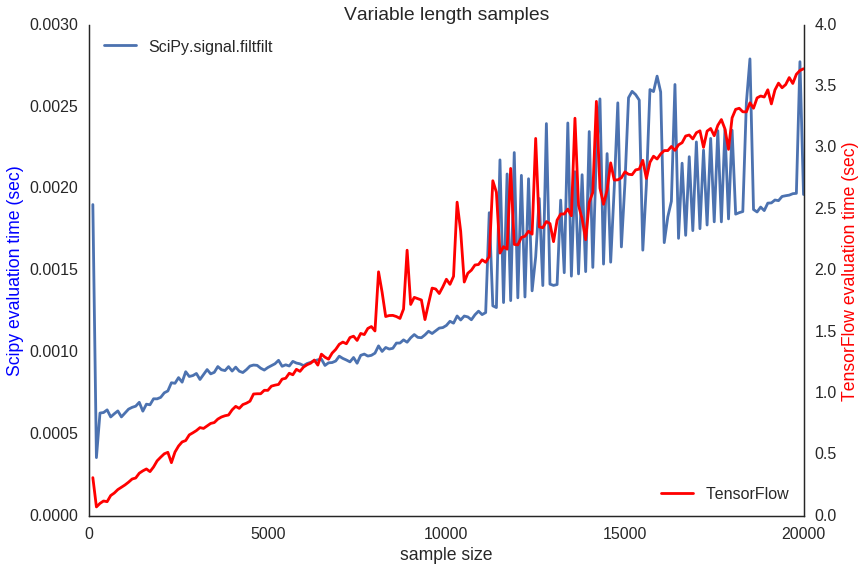
\includegraphics[width=.9\textwidth]{single}
  \caption{Time of evaluating a single sample with a single filter, at different sequence lengths. Later the measurement depicted with the blue line will be used as a baseline representing SciPy's performance on the given task. Notice that for we introduced a new axis for the TensorFlow implementation's time scale, because on single samples the performance of the two methods were not comparable.}
\end{figure}

\section{Batch of samples - Single filter run, with same length samples}

When multiple samples are available at run time, we can speed up the process, by running the same filter process in parallel.
Here we normalized the evaluation time per sample per filter of the SciPy method using the statistics of the previous experiment, since the method allows only processing in sequence, and after reproduced the standard SciPy baseline, to use as a reference point in further benchmarks, e.g. Figure~\ref{fig:batch}.
As we can see in Figure~\ref{fig:batch-tf-only}, the TensorFlow implementation runs in constant time at low batch size, and later starts to increase linearly

\begin{figure}
  \centering
  \begin{floatrow}
    \ffigbox[\FBwidth]{\caption{Comparison to the standardized SciPy baseline with regards to the baseline. The baseline is computed from the normalized average of the different sample length runs from the variable length single sample experiment. We show that with sample length 100, the current implementation only functions better when evaluation above 1500 sample at once.}\label{fig:batch}}{%
      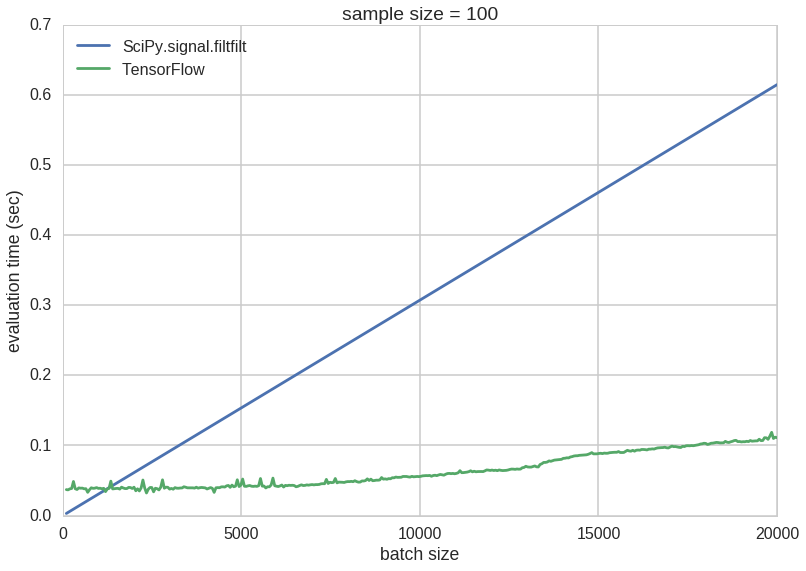
\includegraphics[width=.48\textwidth]{batch}
    }
    \ffigbox[\FBwidth]{\caption{Here only the TensorFlow implementation's evaluation time is depicted without the baseline. It reveals that under 4000 samples the process is nearly constant in time complexity. Above 2000 samples it starts to behave linearly, but it is important to mention that the slope of the fitting linear curve is significantly less steeper than the SciPy baseline.}\label{fig:batch-tf-only}}{%
      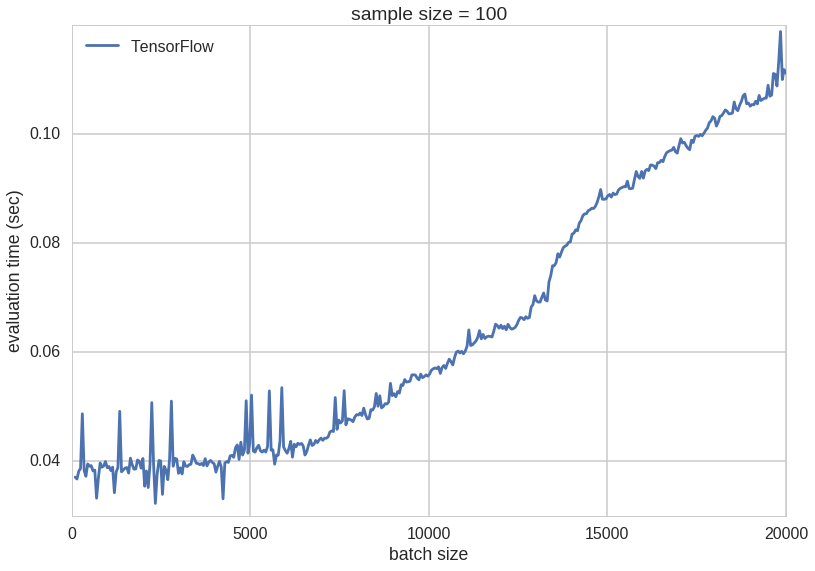
\includegraphics[width=.48\textwidth]{batch-tf-only}
    }
  \end{floatrow}
\end{figure}

% \begin{figure}
%   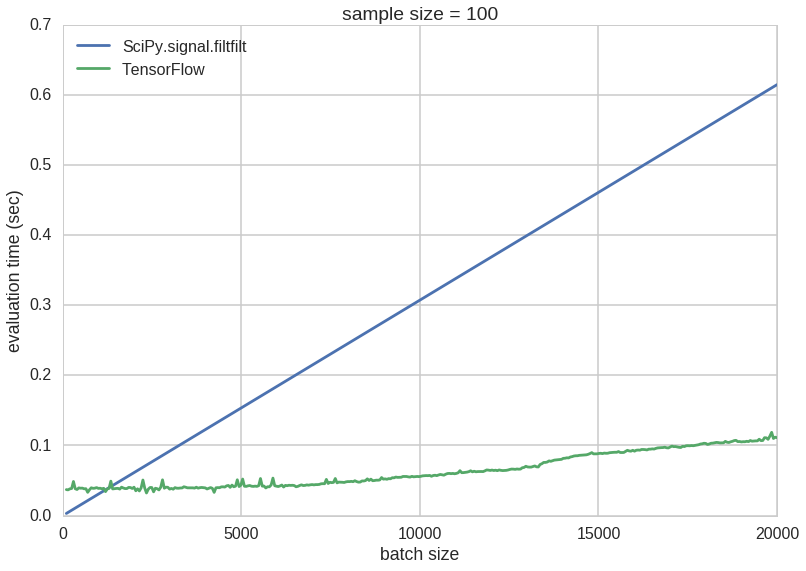
\includegraphics[width=.9\textwidth]{batch}
%   \caption{Comparison to the standardized SciPy baseline with regards to the baseline. The baseline is computed from the normalized average of the different sample length runs from Section~\ref{sec:single}}
%   \label{fig:batch}
% \end{figure}

% \begin{figure}
%   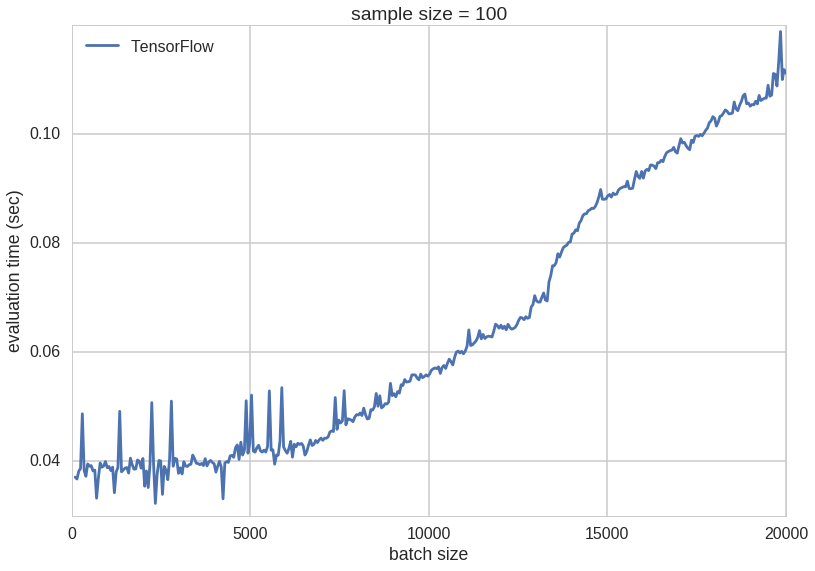
\includegraphics[width=.9\textwidth]{batch-tf-only}
%   \caption{Here only the TensorFlow implementation's evaluation time is depicted without the baseline. It reveals that under 2000 samples the process is nearly constant in time complexity. Above 2000 samples it starts to behave linearly, but it is important to mention that the slope of the fitting linear curve is significantly less steeper than the SciPy baseline.}
%   \label{fig:batch-tf-only}
% \end{figure}

\section{Time per sample}
Finally, we normalized the computation time with regards to the batch size, as a result we have a curve that tells that with fixed sample length at given batch size how much time does it take to evaluate a single entry. For a detailed benchmark see Figure \ref{fig:norm}.

\begin{figure}
  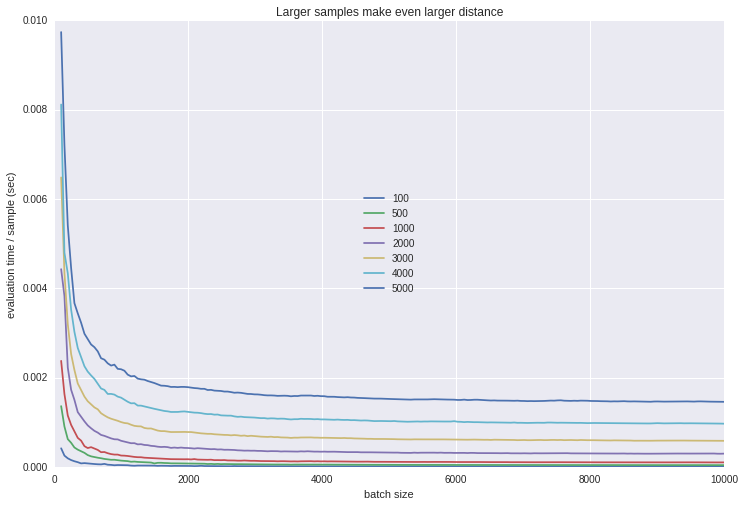
\includegraphics[width=.9\textwidth]{norm}
  \caption{This curve tells that with fixed sample length (different curves on the figure) at given batch size how much time does it take to evaluate a single entry.}
  \label{fig:norm}
\end{figure}
